% TEX STUDIO MAGIC-COMMAND
% !TeX document-id = {21ffa6e2-6c8f-4532-897c-386dc477f19a}
% !TeX root = abstract_final.tex
% !TeX encoding = utf8
% !TeX TXS-program:compile = lualatex -synctex=1 -interaction=nonstopmode -halt-on-error %.tex
% !TeX TXS-program:quick = txs:///compile | txs:///view-pdf-internal --embedded
%%% TeXのファイル名を変えたら ↑ も変えましょう

%%%-------------------------------------------------------------------------
%%% PD3予稿集テンプレート (main.tex)
%%% 作成: 金沢工大・情報工学科・鷹合研究室(2022,01/12)
%%%-------------------------------------------------------------------------

%%%%%%%%%%%%%%%%%%%%%%%%%%%%%%%%%%%%%%%%%%%%%%%%%%%%%%%%%%%%%%%%%%%%%%%%%%%
%                               テーマ,著者情報をここに書き込んでください
%ここから ------------------------------------------------------------------

%%% テーマ番号
\def\THEMEID{1EP6}

%%% タイトル
\def\TITLEJP{Whisperを用いた音素アライメントツールの開発}
\def\TITLEEN{Development of a phoneme alignment tool using Whisper}
\def\CENTERADJ{2.3} % ここを書き換えて,表紙の「プロジェクトテーマ」という文字列がセル中心になるよう調整してください

%%% 教員名
\def\PROFNAME{鷹合 大輔 准教授}

%%% アブストラクト(英文で書く)
% 最低:100ワード,最大:300ワード前後
% 英文部分については,句読点は半角にすること.つまり", "か". "を使う
\def\ABSTRACT{
In recent years, the rapid growth of music distribution services has increased the demand for subtitles for music that synchronize time and lyrics.Therefore, we decided to develop a system that automatically creates subtitles for music.Although Whisper can be used to create subtitles for music, simply inputting music as it is is not accurate enough.Therefore, we constructed a system for sound source separation, a recognition system for silent sections, and a replacement system with correct lyrics. As a result, although not perfect, we were able to handle Whisper with better accuracy and automatically create subtitles for music.
}

%%% キーワード(5個まで)
\def\KEYWORDS{Whisper,Spleeter,音素アライメント,音源分離,編集距離}

%%% 著者リスト
\def\AUTHORS{
\begin{minipage}{13.5cm}
4EP2-20~熊崎 拓人(TAKUTO Kumazaki)
\end{minipage}
}

% テーマ,著者情報ここまで -----------------------------------------------------

%%%%%%%%%%%%%%%%%%%%%%%%%%%%%%%%%%%% 本文
\documentclass{tkglabs}
\begin{document}
\maketitle
\begin{multicols*}{2} % *アスタ付きだとページのバランシングを無効にできる
%本文ここから ------------------------------------------------------------------

\section{はじめに}
近年,音楽配信サービスの急速な増加により,時間と歌詞を同期付けした音楽用の字幕の需要が高まっている.一方,多くの大手カラオケ会社では,歌詞字幕の作成が手動で行われており,非常に時間と労力を必要とする業務となっている.これらの背景から,本プロジェクトでは音楽と正解の歌詞データを入力値として,文字起こしAIであるWhisperを用いて自動で時間同期付きの歌詞データを出力するシステムを開発した.本稿では,歌詞と時間の同期情報が記されているデータのことを「字幕データ」,音声ファイル中の特定の音の始まりと終わりを自動で見つけ出す技術のことを「音素アライメント」と呼ぶ.

\section{システム概要}
本システムの全体の流れを図1に示す.入力値を音楽データと正解歌詞データとし,最初に入力された音楽データからSpleeterを用いて音源分離を行う.その後,音源分離された音楽データから有声区間の抽出を行い,抽出された音源からWhisperを用いて音楽の文字起こしと時間の同期を行う.最後に精度を上げるために正解歌詞データと比較し,間違っている部分を置換し時間と歌詞が同期されたデータが出力されることで終了となる.

\begin{figure} % システムの概要図
\centering
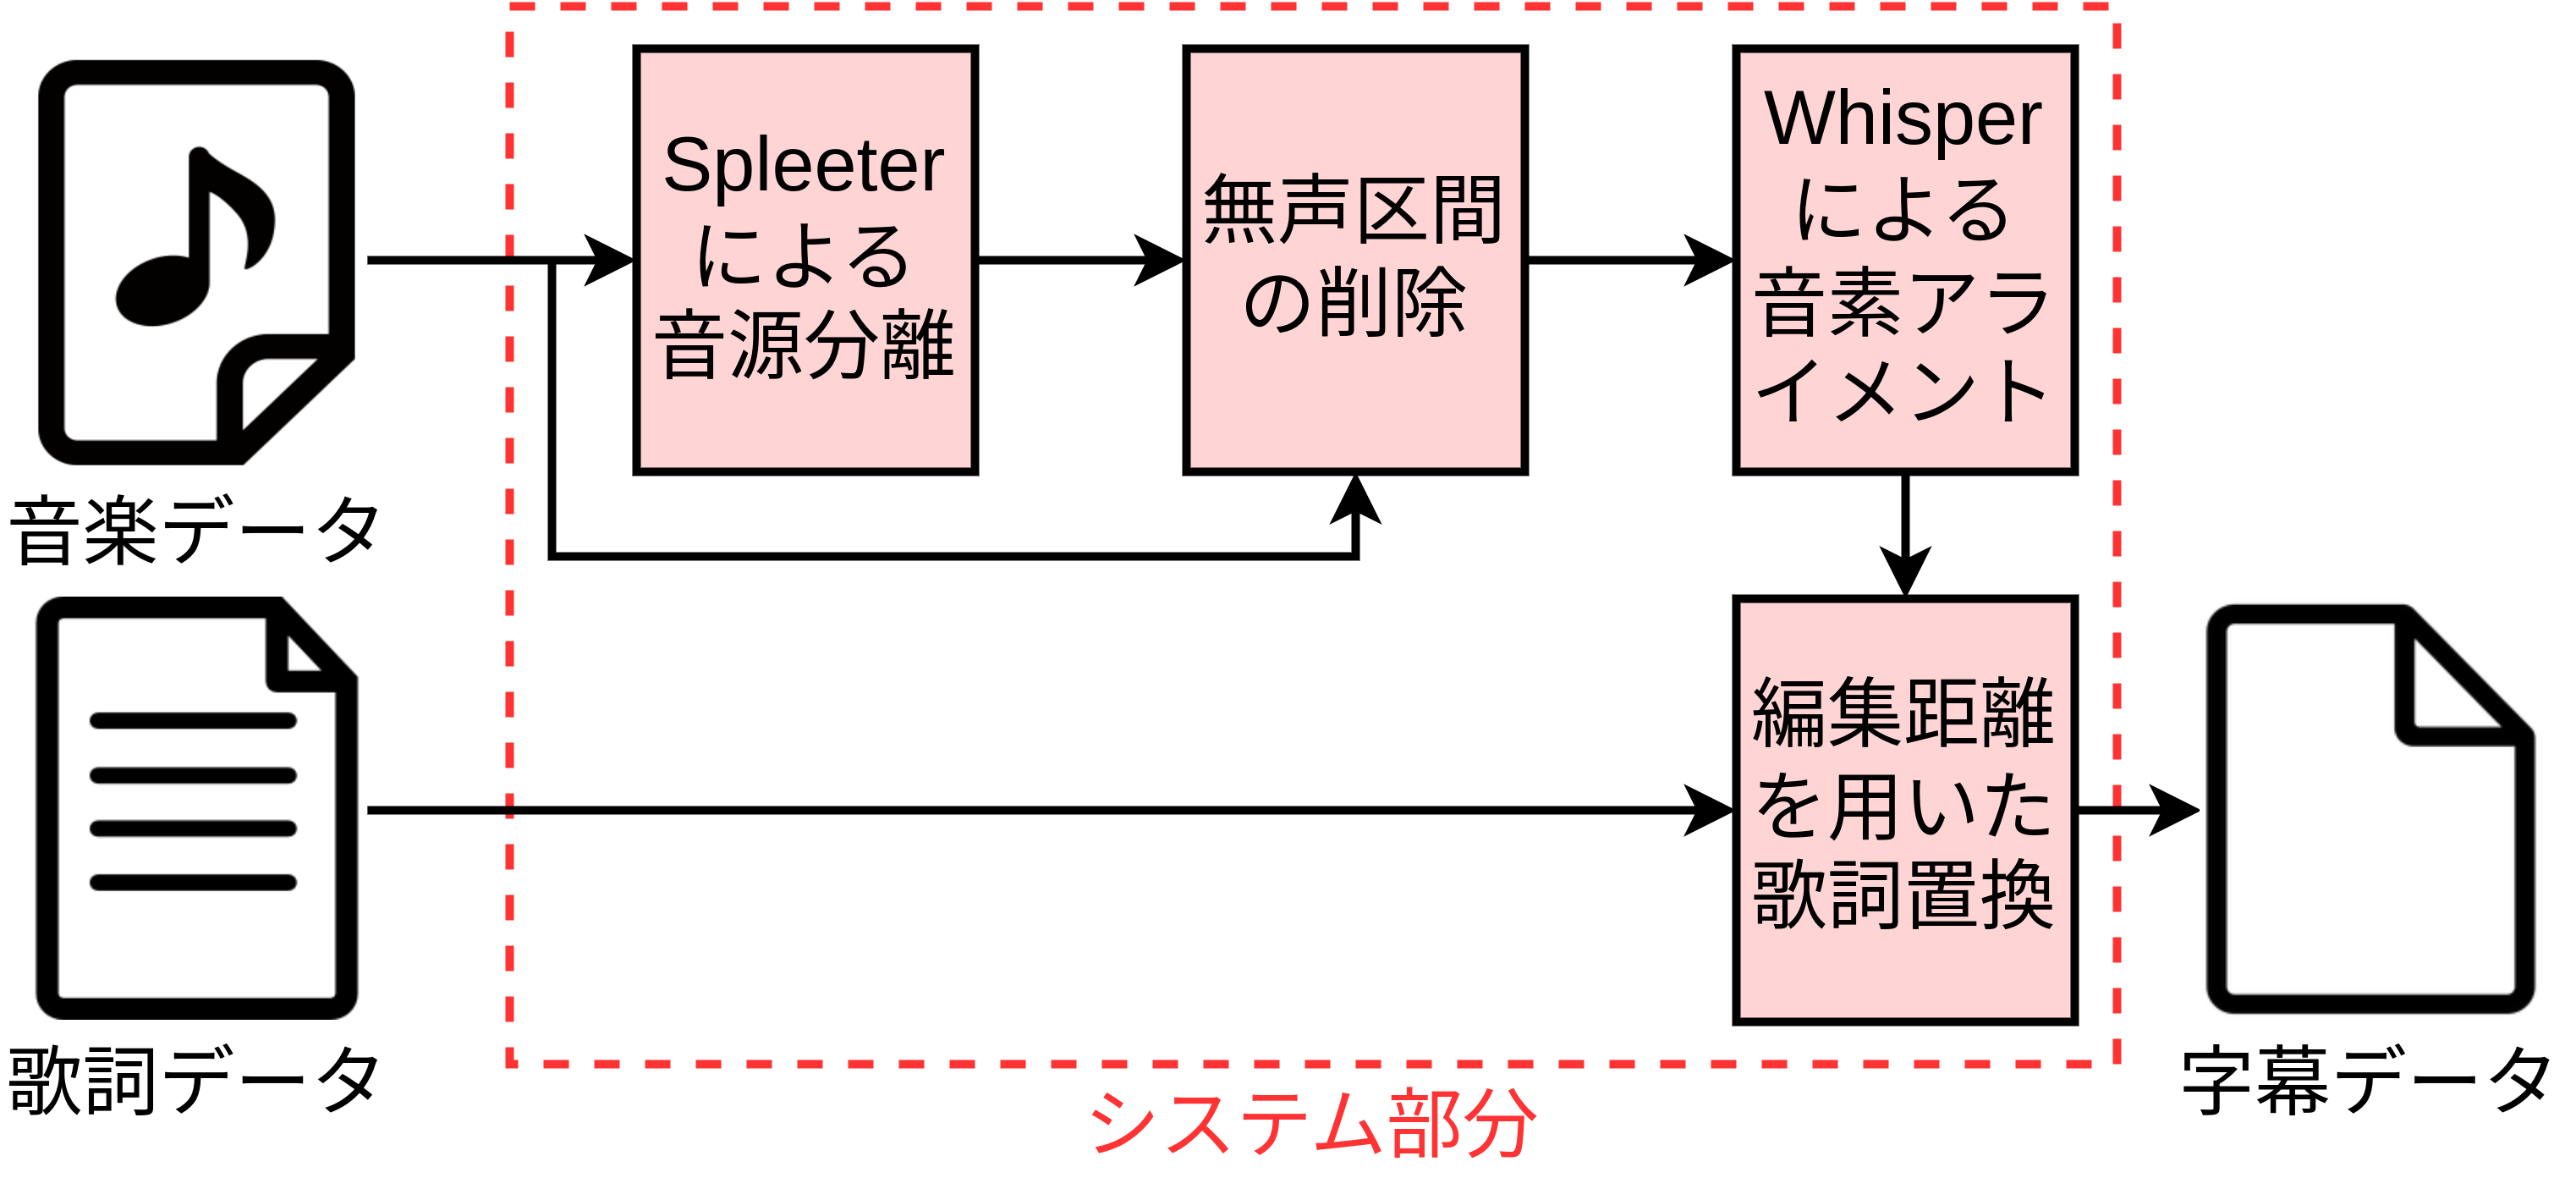
\includegraphics[width=\linewidth]{fig/system_overview2.png}
\figcap{システムの流れ}{Overrall system flow}{FIG_KUJIRA}
\end{figure}

\section{システム詳細}

\subsection{Whisperとは}
Whisperとは,OpenAIが文字起こしサービスとして公開した音声認識モデルである.音楽データをWhisperに入力することで自動で字幕データを作成できるが,音声ファイルをそのまま入力するだけでは精度が不十分であるため,他のシステムを実装することで精度を向上させる.Whisperの具体的な問題点を以下に記す.

\begin{itemize}
\item ボーカルがない部分における誤認識
\item 時間同期の精度が不十分
\item 文字起こしに所々間違いがある
\end{itemize}

\subsection{Spleeterを用いた音源分離}
音源分離とは様々な音が混ざった状態からひとつひとつの音を取り出す技術のことである.今回は音楽の中からボーカルのみを取り出す.SpleeterというPythonライブラリを用いることで簡単に音源分離を行うことができる.

\subsection{無声区間の削除}
ボーカルがない部分で誤認識をするという問題点と時間同期の精度が不十分という問題点を解決するために無声区間を削除する必要がある.librosaというライブラリと音源分離で作成したボーカルのみの音楽データを用いて時間と音量の対応を示したcsvファイルを作成する.次に無声区間を特定するために閾値を設定し,音量の値が閾値より小さい場合はcsvファイルの3列目に0を,閾値以上の場合は0.1を追加する.現在のcsvファイルをグラフで示したものが図2である.無声区間が細かく設定されすぎているため,設定した時間以上無声区間が持続しなかった場合はその無声区間を有声区間に変更する.変更を加えたグラフが図3である.この作成したcsvファイルを使用して無声区間の削除を行う.音源分離後の音楽データに比べ,音源分離前の音楽データのほうがWhisperの文字起こし精度が高いため,音源分離前の音楽データの無声区間を削除する.

\begin{figure} % 無声フラグの画像1
\centering
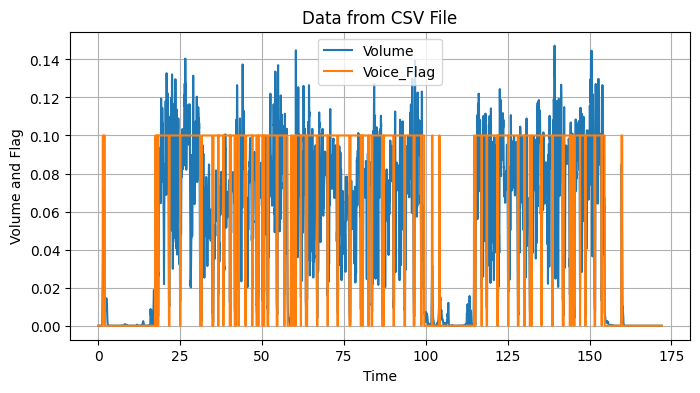
\includegraphics[width=0.95\linewidth]{fig/csv1.png}
\figcap{無声フラグを追加したcsvファイル}{Csv file with silent flag added}{FIG_KUJIRA}
\end{figure}

\begin{figure} % 無声フラグの画像2
\centering
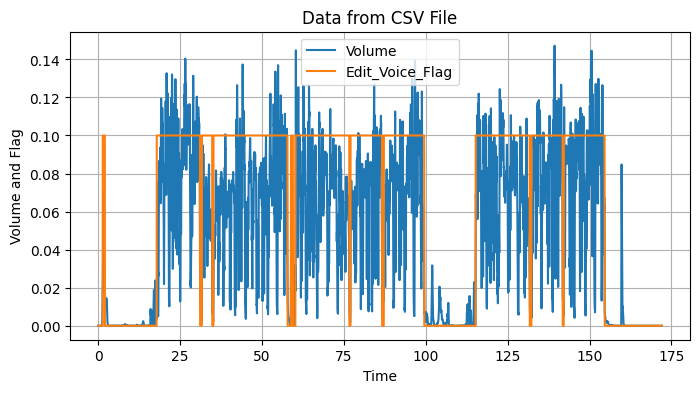
\includegraphics[width=0.95\linewidth]{fig/csv2.png}
\figcap{短い無声フラグを無視したcsvファイル}{Csv file ignoring short silent flag}{FIG_KUJIRA}
\end{figure}

\subsection{Whisperによる音素アライメント}
無声区間を削除した音楽データをWhisperに入力し音素アライメントを行う.Whisperには5つの学習済みモデルがある.本稿では実行時間を考慮して2番目に文字起こし精度が高いmediumモデルを使用する.Whisperに音楽を入力することで文字起こしされた文章とその文章が出現する時間が出力される.この2つの情報を図4のような形式のsrtファイルという字幕データにする.

\begin{figure} % srtファイルの形式
	\centering
	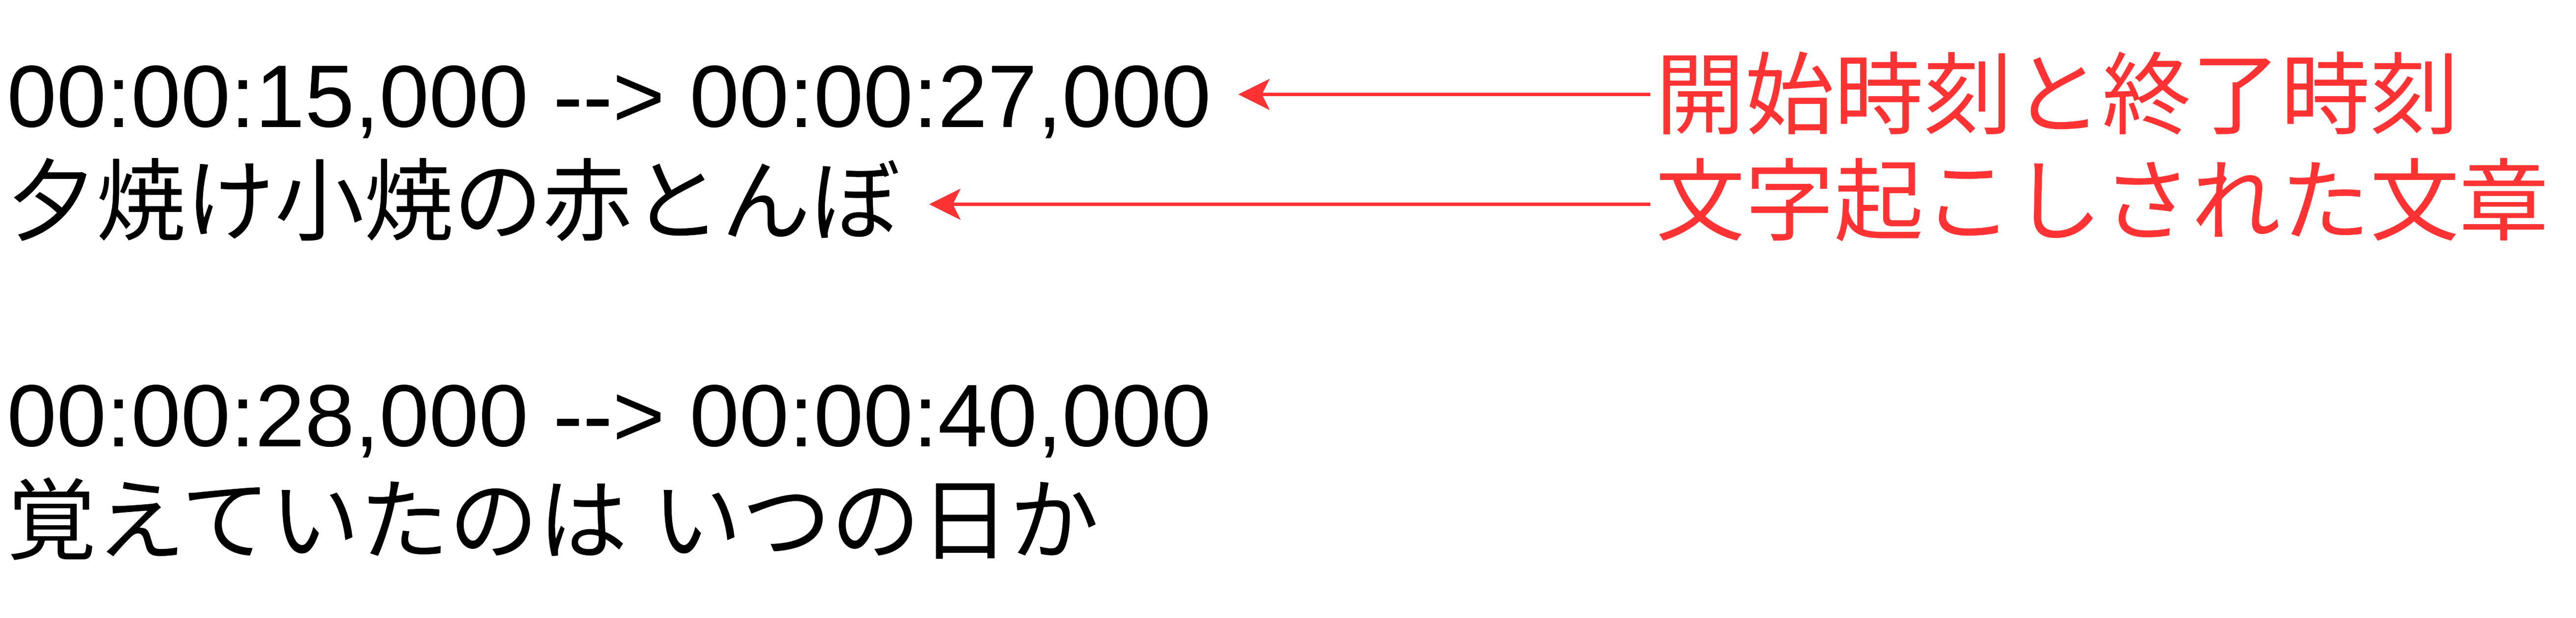
\includegraphics[width=\linewidth]{fig/srt.png}
	\figcap{srtファイルの形式}{Srt file format}{FIG_KUJIRA}
\end{figure}

\subsection{編集距離を用いた歌詞置換}
編集距離とは,2⃣つの文字列がどの程度異なっているかを示す数値であり,語の挿入・削除・置換によって,一方の文字列をもう一方の文字列に変形するのに必要な手順の最小回数で求めることができる.Whisperの文字起こしに所々間違いがあるという問題点を解決するために,正解歌詞と出力された歌詞を比較し,編集距離が最小になるように置換を行う.最初に,入力した正解歌詞データとWhisperで出力された字幕データのそれぞれをMeCabを用いて形態素解析を行い細かい単語や語にする.次に編集距離が最小になるような単語と語の組み合わせを求め,正解歌詞データと字幕データを対応付ける.字幕データの歌詞部分を正解歌詞で置換することによって,より正確な字幕データを作成することができる.

\section{評価実験}

\subsection{実験方法}
テンポの違う音楽を用いて時間同期の精度がどのように変化するかを実験する.歌詞置換が終了した後のsrtファイルから文章を取り出し,手動で正解の開始時刻と終了時刻を入力した新しいsrtファイルを作成する.もとのsrtファイルと新しく作成したsrtファイルを比較して違いがどの程度発生するかを調査する.なお,時間の許容範囲は0.1秒とし,許容範囲内のズレは問題ないものとする.

\subsection{実験結果とその考察}


\section{まとめ}


%% 参考文献(必要に応じて追加)
\begin{thebibliography}{99}
\bibitem{jp2k1} 織田 信長, 明智 光秀, "JPEG2000画像符号化システムにおける係数ビットモデリングと適応算術符号化,"Journal of signal processing(基礎シリーズ), vol.7, no.4, pp.257-266, July 2003.
\bibitem{sdkguide}Parrot, "AR.Drone Developer Guide SDK 2.0"
\bibitem{bk1} "金沢の暮らし", \url{http://www.kanazawa-it.ac.jp}
\bibitem{bk2} 山田 太郎, "金沢の一人暮らし", トンチンカン出版, 2016.
\end{thebibliography}

% 本文ここまで ------------------------------------------------------------------
\end{multicols*} 
\end{document}

